\documentclass{article}
\usepackage{mathrsfs}
\usepackage{bm}
\usepackage{amsmath}
\usepackage{amsthm}
\usepackage{amssymb}
\usepackage{graphicx}
\usepackage{color}
\usepackage{comment}
%\include{macros}
%\usepackage{floatflt}
%\usepackage{graphics}
%\usepackage{epsfig}


\theoremstyle{definition}
\newtheorem{theorem}{Theorem}[section]
\newtheorem{lemma}[theorem]{Lemma}
\newtheorem{proposition}[theorem]{Proposition}
\newtheorem{corollary}[theorem]{Corollary}

\theoremstyle{definition}
\newtheorem*{defition}{Definition}
\newtheorem*{example}{Example}

\theoremstyle{remark}
\newtheorem*{remark}{Remark}
\newtheorem*{note}{Note}
\newtheorem*{exercise}{Exercise}

\setlength{\oddsidemargin}{-0.25 in}
\setlength{\evensidemargin}{-0.25 in} \setlength{\topmargin}{-0.25
in} \setlength{\textwidth}{7 in} \setlength{\textheight}{8.5 in}
\setlength{\headsep}{0.25 in} \setlength{\parindent}{0 in}
\setlength{\parskip}{0.1 in}

\newcommand{\homework}[5]{
\pagestyle{myheadings} \thispagestyle{plain}
\newpage
\setcounter{page}{1} \setcounter{section}{#5} \noindent
\begin{center}
\framebox{ \vbox{\vspace{2mm} \hbox to 6.28in { {\bf
Part~II:~Applications~of~Network~Models~(Spring 2021) \hfill Homework: 04} }
\vspace{6mm} \hbox to 6.28in { {\Large \hfill #1 \hfill} }
\vspace{6mm} \hbox to 6.28in { {\it Lecturer: #2 \hfill} }
\vspace{2mm} \hbox to 6.28in { {\it \hspace{13mm} #3 \hfill} }
\vspace{2mm} \hbox to 6.28in { {\it Student: #4 \hfill} }
\vspace{2mm} } }
\end{center}
\markboth{#1}{#1} \vspace*{4mm} }


\begin{document}

\homework{Lecture 1: Shortest Path Problem}
{Junlong Zhang \hspace{5mm} {\tt zhangjunlong@mail.tsinghua.edu.cn}}
{}
{Zhenyu Jin \hspace{11mm} {\tt jzy20@mails.tsinghua.edu.cn}}{8}

\section*{P1.}
Give the conditions under which Dijkstra algorithm can work. Prove that under these conditions Dijkstra algorithm is correct, that is, we can indeed obtain the shortest paths by using Dijkstra algorithm.
\subsection*{Solution:}
\begin{itemize}
	\item The condition that Dijkstra algorithm can work is non negative weight edge exists in the network.
	\item Prove: \\
Given the condition above, then the distance of point to original must be increasing. According to the formulation given below, $d(i)=min{d(i),d(j)+l(i,j)}$, which point $j$ in the linking set of $i$. Suppose that we have already sort the points in the set, except origin point, the point are $n_0$, $n_1$,$\cdots$, $n_k$, i.e., $d(n_0)$ $\leq$ $d(n_1)$ $\leq$ $\cdots$ $\leq$ $d(n_m)$. Then we have that $d(n_i)=min{l(s,n_i),min_{j<i}{d(n_j)+l(n_i,n_j)}}$ .

\end{itemize}


\section*{P2.}
Give the conditions under which Floyd algorithm can work. Prove that under these conditions Floyd algorithm is correct, that is, we can indeed obtain the shortest paths by using Floyd algorithm.
\subsection*{Solution:}
\begin{itemize}
\item The condition that Floyd algorithm can work include: the network does not contain negative weight cycle.
\item Prove:\\
The Floyd alogrithm can be analogied as dynamic programming, that is, if the shortest path between point $u$ and $v$ pass through the point $w$, then the path of $u$ to $w$ and $w$ to $v$ should be shortest too. \\
Let $G$ be a graph with numbered vertices $1$ to $N$. In the $k^{th}$ step, let shortestPath$(i,j,k)$ be a function that yields the shortest path from $i$ to $j$ that only uses nodes from the set ${1,2,\cdots,k}$. In the next step, the algorithm will then have to find the shortest paths between all pairs $i$,$j$ using only the vertices from ${1,2,…,k,k+1}$.\\
This is the idea of dynamic programming. In each iteration, all pairs of nodes are assigned the cost for the shortest path found so far:
\[
d(i,j,k) = min{d(i,j,k), d(i,k+1,k)+ d(k+1,j,k)}
\]
Hence, that Floyd algorithm can work under the condition that the network has no negative cycle.
\end{itemize}


\section*{P3.}
Give a counterexample for which Floyd algorithm does not work.
\subsection*{Solution:}
\begin{itemize}
\begin{figure}
\centering
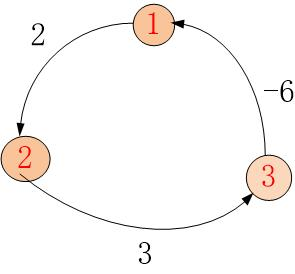
\includegraphics{1.jpg}
\caption{Counterexample of Floyd alogrithm}
\end{figure}
\item The counterexample is given below, since there exsits a negative weight cycle in the network, then the iteration would never end since the total distance could be decrease by each iteration.
\end{itemize}


\section*{P4.}
Analyze the time complexity of Dijkstra algorithm and Bellman-Ford algorithm.
\subsection*{Solution:}
\begin{itemize}
\item The time complexity of Dijkstra algorithm is $O(V^2)$. As depicated in the book $Introduction to Algorithms$, Dijstra can be expressed as,\\

DIJKSTRA(G, w, s)\\
1\quad  INITIALIZE-SINGLE-SOURCE(G, s)\\
2\quad  S ← Ø\\
3\quad  Q ← V[G]               \quad \quad   //V*O(1)\\
4\quad  while Q $\neq$ Ø \\
5\quad \quad      do u ← EXTRACT-MIN(Q)  \quad \quad    // V*O(V), V*O($\lg$ V)\\
6\quad \quad \quad        S ← S$\cup$ \{u\}\\
7\quad \quad \quad       for each vertex v$\in$ Adj[u]\\
8\quad\quad  \quad\quad           do RELAX(u, v, w) \\

\item The time complexity of Bellman-Ford algorithm is $O(VE)$. As depicated in the book $Introduction to Algorithms$, Bellman-Ford can be expressed as,\\

BELLMAN-FORD(G, w, s)\\
1\quad   INITIALIZE-SINGLE-SOURCE(G, s)\\
2\quad   for i  1 to V[G] - 1\quad \quad  //$\theta$(E)\\
3\quad \quad       do for each edge (u, v)  \\
4\quad \quad\quad            do RELAX(u, v, w) \quad \quad //(V-1)$\theta$(E)\\
5\quad   for each edge (u, v)  \\
6\quad  \quad      do if d[v] $\textgreater$ d[u] + w(u, v) \\
7\quad  \quad\quad           then return FALSE \quad \quad // O(E)\\
8\quad   return TRUE\\

\end{itemize}





























\end{document}